\documentclass[a4paper]{article}
\usepackage[utf8]{inputenc}

\usepackage{amsthm}
\usepackage{amssymb}
\usepackage{amsmath}
\usepackage{mathtools}

\usepackage[ruled,vlined]{algorithm2e}
% \usepackage{algorithm}
% \usepackage{algorithmic}
\usepackage{array}
\usepackage{listings}
\usepackage{multirow}

\usepackage[dvipsnames]{xcolor}
\usepackage[toc,page]{appendix}
\usepackage{tikz}
\usepackage{float}
\usepackage{graphicx}
\usepackage{caption}
\usepackage{subcaption}
\usepackage[colorlinks = true,
            linkcolor = blue,
            urlcolor  = blue,
            citecolor = blue,
            anchorcolor = blue]{hyperref}

\graphicspath{ {images/} }
\usepackage[a4paper,width=165mm,top=22mm,bottom=22mm]{geometry}
\setlength{\headheight}{15pt}
% \usepackage[most]{tcolorbox}

\title{Mixed Martial Arts Ontology developed in OWL and SWRL}
\author{Ali Khudiyev}
\date{November 2021}

\begin{document}
\maketitle

\section{Introduction \& Modelling}
\textbf{Mixed Martial Arts (MMA)} is a full-contact combat sport based on striking, grapling and ground fighting. \href{https://www.sportsunfold.com/top-10-best-mma-organizations-promotions}{Top MMA organizations} in the world are \textit{Ultimate Fighting Championship (UFC)}, \textit{Bellator MMA}, \textit{Absolute Championship Akhmat (ACA)} which allow mixed-gender championships by separating male and female events. Such companies gain profit by selling fights as the end-user products each of which goes through the process of organization(i.e., fighter matching, place selection, pay-per-view prices, etc.) and evaluation(i.e., fight winner/drawer, fighter scoring). As in other combat sports, there are divisions among fighters participating in MMA. These divisions are to group fighters in the same weight class to make the championships fair since extra weights can be advantage and/or disadvantage depending on various factors. For example, UFC has the following weight classes\footnote{\url{https://wayofmartialarts.com/ufc-weight-classes-divisions}}:

\begin{table}[H]
	\centering
	\begin{tabular}{c|c}
		\textbf{Weight class} & \textbf{Weight} \\
		\hline
		Heavyweight & 120.2 kg \\
		\hline
		Light heavyweight & 102.1 kg \\
		\hline
		Middleweight & 83.9 kg \\
		\hline
		Welterweight & 77.1 kg \\
		\hline
		Lightweight & 70.3 kg \\
		\hline
		Featherweight & 65.8 kg \\
		\hline
		Bantamweight & 61.2 kg \\
		\hline
		Flyweight & 56.7 kg \\
		\hline
		Strawweight & 52.5 kg
	\end{tabular}
	\caption{UFC Weight Classes}
	\label{tab:ufc_divisions}
\end{table}

Building an ontology is all about observing the relevant existing concepts and the relationships between them. For MMA ontology, there are whole bunch of concepts and relationships, however, 
I will illustrate the ones that are among the most important ones that make MMA what it is. The first concepts that come to the mind in MMA are the notion of 
\textcolor{ForestGreen}{organization} and \textcolor{ForestGreen}{person}. An MMA \textcolor{ForestGreen}{organization} \textcolor{orange}{has a name} and 
\textcolor{orange}{pays} monthly salary to the \textcolor{ForestGreen}{organization workers}. Organization workers can be \textcolor{ForestGreen}{CEO}, \textcolor{ForestGreen}{judges}, 
\textcolor{ForestGreen}{referees}, \textcolor{ForestGreen}{organizers} and \textcolor{ForestGreen}{fighters}. \textcolor{ForestGreen}{Fighters} \textcolor{orange}{participates at} 
\textcolor{ForestGreen}{fights} which is \textcolor{orange}{organized by} \textcolor{ForestGreen}{organizers}, \textcolor{orange}{controlled by} \textcolor{ForestGreen}{referees} and
\textcolor{orange}{judged by} \textcolor{ForestGreen}{judges}. \textcolor{ForestGreen}{Judges} \textcolor{orange}{gives} \textcolor{ForestGreen}{points} to both \textcolor{ForestGreen}{fighters} 
based on which it is decided which \textcolor{ForestGreen}{fighter} \textcolor{orange}{won}/\textcolor{orange}{lost}/\textcolor{orange}{drawed} the \textcolor{ForestGreen}{fight}.
The \textcolor{ForestGreen}{fight} \textcolor{orange}{takes place at} some \textcolor{ForestGreen}{location} and at a specific \textcolor{ForestGreen}{time}, \textcolor{orange}{costs} some 
amount of money which can be \textcolor{orange}{paid by} a \textcolor{ForestGreen}{non organization worker} to \textcolor{orange}{buy} the \textcolor{ForestGreen}{fight}. Every fight 
\textcolor{orange}{has a division} that restricts how much the participating \textcolor{ForestGreen}{fighters} \textcolor{orange}{weigh}. Any two \textcolor{ForestGreen}{fighters} 
have to \textcolor{orange}{have gender} that is either male or female, in other words, (male vs female) match is impossible due to unfairness. The \textcolor{ForestGreen}{organization} 
have certain age restrictions for its \textcolor{ForestGreen}{workers} and also \textcolor{orange}{pays bonus} money to a winning \textcolor{ForestGreen}{fighter}.
The whole information can be represented as the knowledge graph shown below:

\begin{figure}[H]
	\centering
	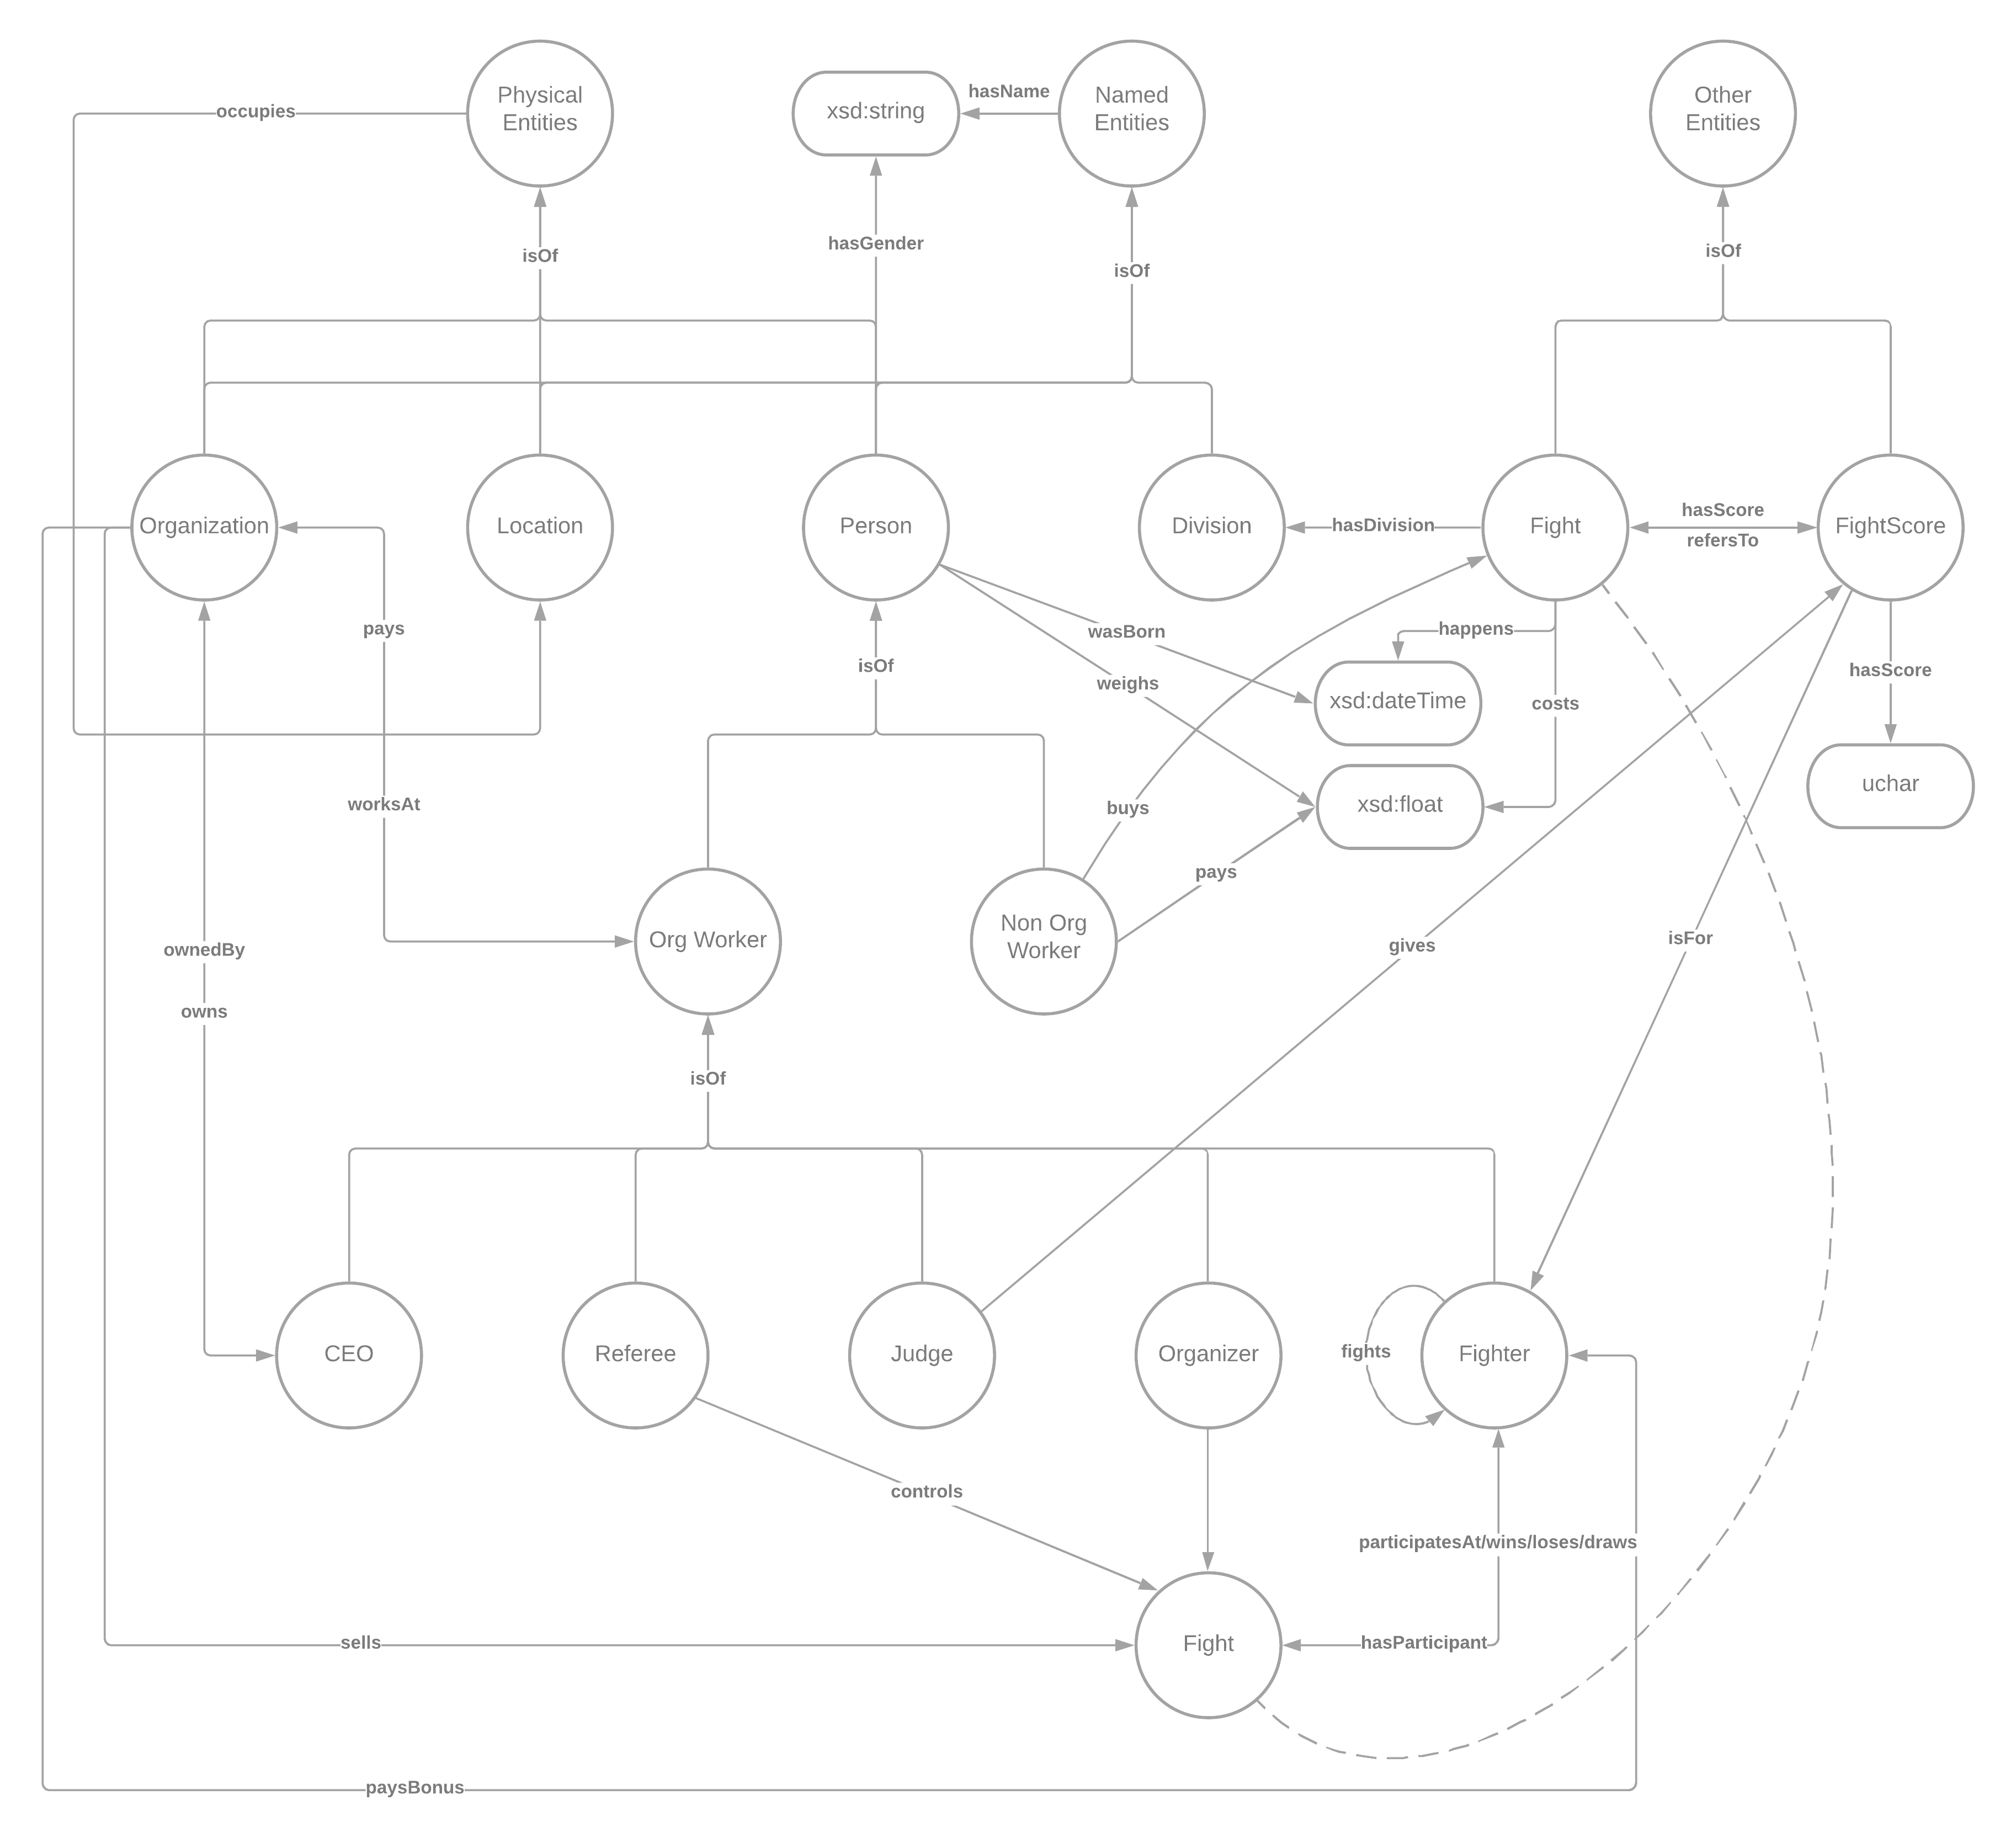
\includegraphics[width=0.75\textwidth]{resources/mma_onto.png}
	\caption{MMA Ontology Diagram}
	\label{fig:mma_ontology}
\end{figure}

However, it is not enough to represent the whole just by using OWL alone and in fact, there are rules which represent some of the relationships hidden in the OWL graph. 
There are several rules that are among the most relevant ones as far as this project concerns and they are shown below in DL.

\begin{equation}	
	Fight \sqsubseteq =2hasParticipant.Fighter
	\label{formula:fight_participants}
\end{equation}

% \begin{equation}
% 	\begin{split}
% 		\forall x (Fight(x) \implies& \exists y \exists z (\text{differentFrom}(y, z) \land \\
% 									& \text{Fighter}(y) \land \text{Fighter}(z) \land \\ 
% 									& \text{participatesAt}(y, x) \land \text{participatesAt}(z, x))
% 	\end{split}
% 	\label{formula:fight_participants}
% \end{equation}

\begin{equation}
	\begin{split}
		\text{Fight}(f) &\land \text{Fighter}(x) \land \text{Fighter}(y) \land \text{participatesAt}(x, f) \\
						&\land \text{participatesAt}(z, x) \land \text{differentFrom}(x, y) \implies a = b
	\end{split}
	\label{formula:fighter_weights}
\end{equation}

% \begin{equation}
% 	\begin{split}
% 		\forall x \forall y \forall z (&\text{Fight}(x) \land differentFrom(y, z) \land \text{participatesAt}(y, x) \\
% 									   &\land \text{participatesAt}(z, x) \implies \text{weight}_{y} = \text{weight}_{z})
% 	\end{split}
% 	\label{formula:fighter_weights}
% \end{equation}

\begin{align}
	\forall x \forall y (\text{Fighter}(x) \land \text{Fighter}(y) \land \text{wins}(x, y) \implies \text{loses}(y, x)) \\
	\forall x \forall y (\text{Fighter}(x) \land \text{Fighter}(y) \land \text{draws}(x, y) \implies \text{draws}(y, x)) \\
	\forall x (\text{Fighter}(x) \implies (\text{wasBorn}_{x} \geq 1970)) \\
	\forall x (\text{Referee}(x) \implies (\text{wasBorn}_{x} \geq 1950)) \\
	\forall x (\text{Judge}(x) \implies (\text{wasBorn}_{x} \geq 1950))
	\label{formula:mma_axioms}
\end{align}

Formula \ref{formula:fight_participants} indicates that any fight has to have exactly 2 participating fighters while \ref{formula:fighter_weights} is to say that every couple of fighters 
who has fought against each other have to weigh the same which is due to the division rules of MMA. Formulas \ref{formula:mma_axioms} are to restrict organization worker's ages, ?

\section{Implementation in Prot\'eg\'e}
The implementation goes through several stages: \textit{creating class hierarchy and defining class equivalance(s)/ subsumtion(s)/ disjuntion(s)}, \textit{defining relations}, 
\textit{defining SWRL rules} and finally \textit{creating individuals}. The class hierarchy is created by simply creating concepts used in the ontology and the class properties such as 
equivalance\footnote{Although equivalance is rarely used as it is mainly for merging two separately developed ontologies, there are classes which make it relevant to use it in this project.}, 
subsumtion, disjuction between them are defined within the scope of the same classes. Relations are to link different concepts with their relevant predicates and have properties(i.e., 
reflexivity, transivity, etc.) as well. These 2 steps are what can be done using only OWL and they are carefully developed to avoid unintentional situations later on. The third step, 
which is defining SWRL rules, is developed by using SWRLTab in Prot\'eg\'e and tested with the OWL individuals that are created at the final development step of the ontology.

\subsection{Creating and Defining Classes}
There are several concepts(classes) in this ontology:

\begin{itemize}
	\item Organization
	\item Location
	\item Person
	\begin{itemize}
		\item Organization Worker
		\begin{itemize}
			\item CEO
			\item Judge
			\item Referee
			\item Organizer
			\item Fighter
		\end{itemize}
		\item Non Organization Worker
	\end{itemize}
	\item Fight
	\item FightScore
\end{itemize}

\begin{align}
	\text{OrgWorker} \cup \text{NonOrgWorker} &= \text{Person} \\
	\text{OrgWorker} \cap \text{OrgWorker} &= \emptyset
	\label{eq:class_axioms}
\end{align}

\subsection{Defining Relations}
A relation in logic has some arity, which is usually called k-ary relation. When $k$ is 1, it is called unary and when $k$ is 2, it is called binary relation. In Prot\'eg\'e, only binary relations are 
developed and therefore, we give off some level expressiviness as a trade-off with computation complexity. Due to such expressivity, any relation with more than arity 2 has to be reformulated with the 
help of additional concepts and relations. It is the same case with the classes \textit{Fight}, \textit{FightScore} and \textit{Fighter} in this project; as it is impossible to have a 3-ary relation 
describing a \textit{score} of \textit{fighter} in a particular \textit{fight}. There are also several properties of binary relations such as functional, symmetric, reflexive, transtive and so on. 
These properties are also used in the developement when it is relevant and necessary to avoid illogical KB and/or inferences.

\begin{table}[H]
	\centering
	\begin{tabular}{|c|c|c|c|c|}
		\hline
		\textbf{Relation} & \textbf{Domain} & \textbf{Range} & \textbf{Type} & \textbf{Description} \\
		\hline
		hasName & Thing & string & functional & Any concept has a name \\
		\hline
		sells & Organization & Fight & regular & Organization sells fights \\
		\hline
		buys & NonOrgWorker & Fight & regular & Non organization worker can buy fights \\
		\hline
		pays & NonOrgWorker & float & functional & Non organization worker pays to buy fights \\
		\hline
		participatesAt & Fighter & Fight & regular & Fighter participates at a fight by fighting \\
		\hline
		wins & Fighter & Fighter & inverse(loses) & Fighter can win another fighter \\
		\hline
		loses & Fighter & Fighter & inverse(wins) & Fighter can lose to another fighter \\
		\hline
		draws & Fighter & Fighter & regular & Fighters can draw \\
		\hline
	\end{tabular}
	\caption{Ontology Relations}
	\label{tab:relations}
\end{table}

\subsection{Defining SWRL Rules}

\subsection{Creating Individuals}

\begin{table}[H]
	\centering
	\begin{tabular}{|c|c|c|}
		\hline
		\textbf{Individual} & \textbf{Asserted} & \textbf{Inferred} \\
		\hline
		Org & Organization & \\
		\hline
		OrgCEO & Person & \\
		\hline
		OrgFighter1 & Fighter & \\
		\hline
		OrgFighter2 & Fighter & \\
		\hline
		OrgFighter3 & Fighter & \\
		\hline
		OrgFighter4 & Fighter & \\
		\hline
		Fight1 & Fight & \\
		\hline
		Fight2 & Fight & \\
		\hline
		FightScore1\_1 & FighScore & \\
		\hline
		FightScore1\_2 & FighScore & \\
		\hline
		FightScore2\_1 & FighScore & \\
		\hline
		FightScore2\_2 & FighScore & \\
		\hline
	\end{tabular}
	\caption{Individuals}
	\label{tab:individuals}
\end{table}

% bonus section
\subsection{SPARQL Queries}
\ldots

\section{Reasoning with Pellet}
\ldots

\section{Evaluation \& Conclusion}
OWL and SWRL help us to create ontologies with certain subset of first order logic that makes the inference decidable. To do so, it sacrifices some sort of expressiviness that could be otherwise used to 
develop certain ontologies(e.g. an ontology that requires creation of new individuals under some conditions). Another type of problem may arise when trying to represent object states that is dynamic over time 
since there is no concept of time in OWL and SWRL. Consider we want to simulate \textit{Conway's Game of Life}\footnote{\url{https://en.wikipedia.org/wiki/Conway\%27s\_Game\_of\_Life}} by using SWRL rules. 
Since there are cells that are either alive or dead depending on the state of the neighbours, it is not very intuitive to represent a cell which can transform from being dead to alive or vice versa as 
iterations are developed. However, we could still simulate the GoL by representing the concept of time/iteration as an extra dimension. After thinking on the proper way of representing time, I settled in the 
following representation: \textit{each individual cell has its own (current) time or iteration rather than a global notion of time}. This decision comes from the realization that rules can be applied 
randomly when relevant which interrupts the synchronization between cell states and the iteration that they are in. So, rather than having a global notion of iteration, each cell has its own sense of 
iteration which is developed as the reasoner processes or does some transformation upon the cell.

\begin{figure}[H]
	\centering
	\begin{align*}
	\text{Time}&(T) \\
	\text{AliveCell}&(c1) \\
	\text{DeadCell}&(c2) \\
	\text{DeadCell}&(c3) \\
	\text{AliveCell}&(c4) \\
	\text{Time}(T) \land \text{hasValue}(T, t) &\implies \text{hasValue}(T, t+1)
	\end{align*}
	\caption{Notion of global time}
\end{figure}

\begin{figure}[H]
	\centering
	\begin{align*}
	Cell&(c1) \\
	Cell&(c2) \\
	Cell&(c3) \\
	Cell&(c4) \\
	isLiveAt&(c1, 1) \\
	isLiveAt&(c2, -1) \\
	isLiveAt&(c3, -1) \\
	isLiveAt&(c4, 1) \\
	\text{Cell}(c) \land \text{isLiveAt}(c, t) \land \text{hasSufficientNeighbours}&(c, t) \land \text{isNegative}(t) \implies \text{isLiveAt}(c, 1-t) \\
	\text{Cell}(c) \land \text{isLiveAt}(c, t) \land \text{hasSufficientNeighbours}&(c, t) \land \text{isPositive}(t) \implies \text{isLiveAt}(c, 1+t) \\
	\text{Cell}(c) \land \text{isLiveAt}(c, t) \land \text{hasInsufficientNeighbours}&(c, t) \land \text{isNegative}(t) \implies \text{isLiveAt}(c, -1+t) \\
	\text{Cell}(c) \land \text{isLiveAt}(c, t) \land \text{hasInsufficientNeighbours}&(c, t) \land \text{isPositive}(t) \implies \text{isLiveAt}(c, -1-t) \\
	\text{Cell}(c) \land \text{hasNeighbour}(c, c1) \land \text{isLiveAt}(c1, t) \land \dots \land &\text{ isPositive}(t) \implies \text{hasSufficientNeighbours}(c, t) \\
	\text{Cell}(c) \land \text{hasNeighbour}(c, c1) \land \text{isLiveAt}(c1, t) \land \dots \land &\text{ isPositive}(t) \implies \text{hasInsufficientNeighbours}(c, t)
	\end{align*}
	\caption{Notion of local time}
\end{figure}

The predicate \lstinline{isLiveAt(cell, t)} represents an alive cell when $t>0$ and a dead cell when $t<0$. The analogy here is that time is bidirectional; positive time represents the time in our world 
and negative time represents the time in afterlife. So, \lstinline{isLiveAt(cell, 3)} indicates that the cell is alive at the iteration 3 and \lstinline{isLiveAt(cell, -4)} means that the cell is alive 
at the iteration 4 in afterlife, in other words, the cell is dead at iteration 4 (in our world). A cell is alive in our world when it is dead in the afterlife and vice versa. This representation avoids 
the creation of new cells (as it is also prohibited in DL) and helps us to illustrate the notion of iteration/time. However, the above shown rules are not the only ones required to build such interesting 
ontology and the missing pieces that I have not intentionally mentioned is the formulas describing \lstinline{hasSufficientNeighbours}(cell, t) and \lstinline{hasInsufficientNeighbours}(cell, t); these 
are also updates through the process. In fact, \lstinline{hasSufficientNeighbours(cell, t)} is updated to indicate that if cell has sufficient number of neighbours at iteration $t$ to keep living 
(if live before) or turn to an alive cell (if dead before) at the consequent($t+1$) iteration. It is the opposite case for \lstinline{hasInsufficientNeighbours(cell, t)} which is updated to indicate 
whether a cell has less or more than enough live neighbours at the iteration $t$.
\end{document}
